\begin{frame}
	\frametitle*{Inhalt}
	\tableofcontents
\end{frame}

\section{Aufgabe}
\begin{frame}
	\frametitle*{Aufgabe}
	\begin{itemize}
		\item Erstellung eines REST-Webservices
		\item Szenario: Bikesharing
		\item Implementierung in PHP
		\item Vertiefung im Bereich Sicherheit
	\end{itemize}
\end{frame}

\section{Vorgehen}
\begin{frame}
	\frametitle*{Vorgehen}
	\begin{itemize}
		\item URLs definiert unter denen Ressourcen erreichbar sind
		\item zu jeder Ressource Anfrage- und Antwort-Parameter festgelegt
		\item Webservice implementiert
		\item Client-Anwendung implementiert
	\end{itemize}
\end{frame}

\section{URLs}
\begin{frame}
	\frametitle*{URLs}
	\begin{figure}
		\centering
		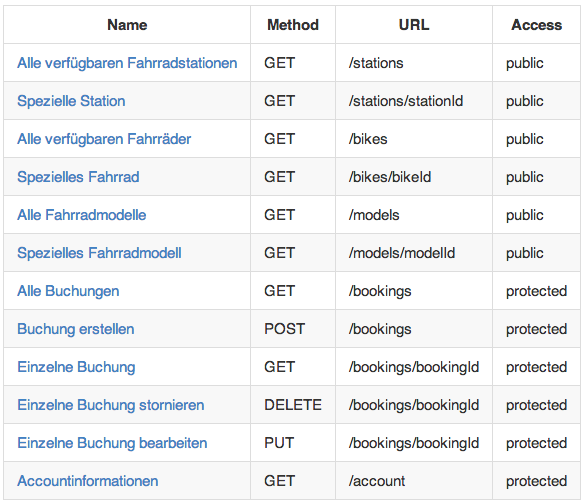
\includegraphics[height=50mm]{pics/endpoints.png}
	\end{figure}
\end{frame}

\section{Anfrage- und Antwort-Parameter}
\begin{frame}
	\frametitle*{Anfrage- und Antwort-Parameter}
	\begin{itemize}
		\item Beschreibung der Paramater und dessen Format
		\item Festlegen welche verpflichtend sind und welche optional
	\end{itemize}
	\begin{figure}
		\centering
		
\includegraphics[height=4mm]{pics/request_example.png}
	\end{figure}
	\begin{figure}
		\centering
		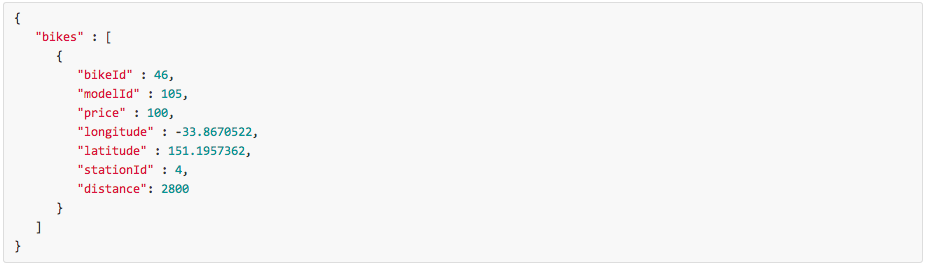
\includegraphics[height=28mm]{pics/response_example.png}
	\end{figure}
\end{frame}

\section{Webservice}
\begin{frame}
	\frametitle*{Webservice}
	\begin{itemize}
		\item Verwendung des Slim-Frameworks
		\begin{itemize}
			\item sehr einfaches und kleines Framework
			\item durch Middlewares erweiterbar (bereits mehere für OAuth vorhanden)
			\item umfangreiche Dokumentation
		\end{itemize}
	\end{itemize}
\begin{figure}
		\centering
		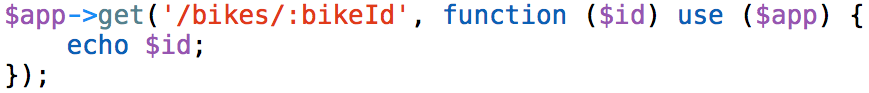
\includegraphics[height=5mm]{pics/slim.png}
	\end{figure}
\end{frame}

\section{Client-Anwendung}
\begin{frame}
	\frametitle*{Client-Anwendung}

\end{frame}

\section{Weiteres Vorgehen}
\begin{frame}
	\frametitle*{Weiteres Vorgehen}
	\begin{itemize}
		\item Client-Anwendung vervollständigen
		\item Authentifizierung mittels OAuth hinzufügen
		\item Verwendung von HTTPS
	\end{itemize}
\end{frame}

\section{Quellen}
\begin{frame}
	\frametitle*{Quellen}
	\begin{itemize}
		\item \url{slimframework.com}
	\end{itemize}
	%\bibliography{../literatur}
\end{frame}
